\documentclass{article}
\usepackage[T1]{fontenc}
\usepackage{lmodern}
\usepackage{graphicx}
\usepackage{amsmath,amssymb}
\usepackage[a4paper,margin=2cm]{geometry}
\usepackage[absolute,overlay]{textpos}
\setlength{\TPHorizModule}{1mm}
\setlength{\TPVertModule}{1mm}
\usepackage[indonesian]{babel}
\usepackage{hyperref}
\setlength{\emergencystretch}{2em}
% unit: Halaman 9

\begin{document}

% === Halaman 9 (llm) ===

\vspace{178.20mm}

Sumber asli dari dokumen FIPS-PUB

% deskripsi: Diagram alir struktur algoritma enkripsi DES (Data Encryption Standard) yang menunjukkan proses permutasi awal, 16 ronde transformasi Feistel dengan kunci $K_1$ hingga $K_{16}$, dan permutasi akhir.
% bbox normalisasi: [0.3020, 0.3800, 0.6850, 0.9800]
\begin{textblock*}{80.43mm}(63.42mm,112.86mm)
\noindent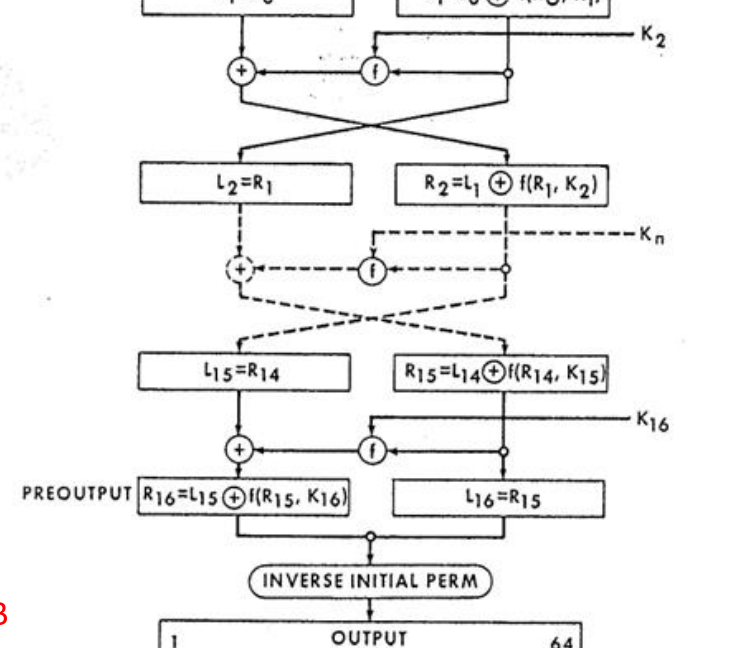
\includegraphics[width=80.43mm,height=178.20mm]{../../images/llm/page_009_img_01.png}%
\end{textblock*}

\end{document}
